% $ based on Id: sample_english-v1.2.tex,v 1.2 2007/04/12 21:05:22 zlb Exp $
% $Id: sample_english.tex 6 2011-01-24 13:13:33Z hsqi $

\documentclass[english]{cccconf}
%\documentclass[usemulticol,english]{cccconf}
\usepackage[comma,numbers,square,sort&compress]{natbib}
\usepackage{epstopdf}
\usepackage{amsmath}
\usepackage{pstricks,pst-node,pst-tree,pstricks-add}
\usepackage{graphics,graphicx}
\usepackage{amssymb}

\newtheorem{condition}{Condition}
\newtheorem{assumption}{Assumption}
\newtheorem{colloary}{Colloary}
\newtheorem{theorem}{\bf Theorem}
\newtheorem{proposition}{Proposition}
\newtheorem{lemma}{Lemma}
\newtheorem{example}{Example}
\newtheorem{notation}{Notation}
\newtheorem{definition}{\bf Definition}
\newtheorem{remark}{Remark}


\begin{document}



\title{Fully Distributed Consensus Control for Nonlinear Multi-agent Network with Extended State Observer}

\author{Shaopan Guo and
        Zhongkui Li}

% Note: the first argument in the \affiliation command is optional.
% It defines a label for the affiliation which can be used in the \aref
% command. If there is only one affiliation for all authors, then the
% optional argument in the \affiliation command should be suppressed,
% and the \aref command should also be removed after each author in
% \author command, in this case the affiliation will not be numbered.

\affiliation{State Key Laboratory for Turbulence and Complex Systems, Department of Mechanics and Aerospace Engineering, Peking University, Beijing 100871, P.~R.~China
        \email{guoshaopan@pku.edu.cn}}

\maketitle

\begin{abstract}
The consensus problem of networks for nonlinear agents is covered in this paper. Built on linear extended state observer (LESO), a distributed consensus protocol is proposed and designed. Compared with the previous related papers, our main contribution is that the proposed consensus protocol is fully distributed by using a node-based adaptive method, which does not need any global information about the communication topology and is independent of the network's scale. Moreover, a sufficient condition is derived to ensure that the consensus errors of the nonlinear multi-agent systems converge to zero eventually. Lastly, a simulation example is submitted to demonstrate the effectiveness of the theoretical consequences.



\end{abstract}

\keywords{extended state observer, multi-agent systems, adaptive control, consensus, distributed control, }

% Please remove or comment out the following line if the footnote is not necessary
%\footnotetext{This work was supported by the National Natural Science Foundation of China under grants 61473005 and 11332001 and a Foundation for the Author of National Excellent Doctoral Dissertation of PR China. Corresponding author: Zhongkui Li.}

\section{Introduction}

In last two decades, there is surging interest on the research of the multi-agent system due to its huge potential applications in lots of scientific communities, which is including but not limited to sensor networks, formation flying, and cooperative surveillance \cite{Li2010Consensus,Olfati2007Consensus,Ren2007Information}. All of these applications get benefit by an in-depth study on the consensus problem, which makes consensus problem still a research hotspot up to now. From different perspectives, consensus problem and its closely related problems have been addressed by many pioneers; see \cite{Olfati2004Consensus,Ding2016Distributed,Li2016Distributed,Ren2005Consensus,Li2013Consensus} and reference therein.  

However, most existing works by now focus on the multi-agent with linear dynamics. But we all know that major physical plants are both nonlinear and highly uncertain in the real world, which means the linear system is just a small part or simplification of the actual systems \cite{Zheng2008On}. The active disturbance rejection control (ADRC), which was introduced by Han  in 1995 built on extended state observer (ESO)\cite{Gao2015Active}, is a powerful tool to tackle this problem\cite{Han2009From}.
ESO, which is operating as an estimator, takes a key position in the ADRC. The core idea of ESO is that it regards the total nonlinear part of the system and external disturbance as an augmented state and then this augmented state with the other states of the system can be estimated via the observer on-line. Compared with the typical disturbance attenuation methods like robust control (RC), sliding model control (SMC), and internal model control (IMC), ESO can react directly and extremely rapid with the strong disturbance\cite{Li2014Disturbance}, which is really important in the applications of industrial and military fields, and attracts more and more attention and discussion in the scientific communities \cite{Guo2012,Sun2017Sampled,Wang2016Consensus}.

Recent years, many researchers have tried to introduce this powerful tool to solve the disturbance rejection  and internal uncertainty problems faced in multi-agent systems and got some exhilarating results \cite{XiangyuWangTAC2017,DongCCC2017,Qin2014}. \cite{XiangyuWangTAC2017} presents a distributed active anti-disturbance consensus protocol for the high-order multi-agent system with mismatched disturbance. In \cite{DongCCC2017}, the time-varying formation tracking problems are studied based on ESO, while it only gets a bounded result of the tracking errors. In \cite{Qin2014}, it studies the formation control problem with switching topologies using linear extended state observer (LESO), but the agent dynamics are limited to double-integrator. Moreover, the design of distributed control protocols in these aforementioned works need the information of the smallest nonzero eigenvalue of the Laplacian matrix for corresponding communication graphs. However, it is a global information in the sense that each agent can compute it only if it know the entire communication graph. So their control protocols are not fully distributed, which limits their application to the real world problems. 

Motivated by the limitation of existing works mentioned above, we investigate the consensus problem for nonlinear multi-agent system where each agent does not have the ability to know the knowledge of the entire communication graph. To address this problem, we first construct a linear extended state observer built on their own output information which can estimate the agents' nonlinear dynamics and external disturbance at the same time. By using the extended state observers' states, a distributed node-based adaptive consensus protocol is constructed to reach consensus and meanwhile to reject the impact of the external disturbance. Then a practical method is proposed to determine the gain matrix of the control law.

Our main contributions lie in the following aspects. %compared with the previous related works \cite{XiangyuWangTAC2017,DongCCC2017,Qin2014}. \cite{XiangyuWangTAC2017}. 
First, we propose a node-based adaptive consensus control protocol for nonlinear multi-agent system in the presence of external disturbance. We use extend state observer to realize the on-line estimation for both the nonlinear dynamics of the agents and the external disturbance, where the agent dynamics are not limited to double-integrator compared with \cite{Qin2014}. Moreover, a sufficient condition is derived to ensure that the consensus errors of the nonlinear multi-agent systems converge to zero eventually, while \cite{DongCCC2017} only gets a bounded result of the tracking errors. Then, using a node-based adaptive control law ensures that only local information is needed to construct control protocols, which is not be done in \cite{XiangyuWangTAC2017,DongCCC2017,Qin2014}.  Finally, we present a numerical simulation to show the effectiveness of the theoretical results.

The reminder of the paper is structured as follows: in section 2, the description of the system dynamics, the extended state observer (ESO) form and the problem statement are introduced. In section 3, we will show our main results and the design method of the fully distributed node-based adaptive control law and the sufficient condition for consensus based on Lyapunov theory. A numerical simulation is presented in section 4 to demonstrate the effectiveness of the theoretical consequences. And some remarks and conclusions are outlined in section 5. 

\begin{notation}

The set of $n \times m$ real matrices is denoted by $\mathbf R^{n \times m}$. $\Vert \cdot \Vert$ represents the Euclidean norm of real vectors while $\vert \cdot \vert$ represents the absolute value of scalars. $\lambda_{min}$ and $\lambda_{max}$ denote the smallest and largest eigenvalue of a matrix A. For a symmetric $Q \in \mathbf R^{n \times n}$, we say $Q > 0$ if $x^{T} Q x > 0$ for $x \neq 0$. The subscript $T$ represents the transpose for real matrices. Matrix $I_p \in R^{p \times p}$ means the identity matrix. $\mathbf 1_{\mathbf N}$ represents $1 \times N$ column vector of all ones. Denote by $diag(A_1, \cdots , A_N)$ a block-diagonal matrix with elements $A_i$ , $i = 1, \cdots, N$ on its diagonal.  A function $f: \mathbf R^n \to \mathbf R^m$ is called to be Lipschitz if for any $x \in \mathbf R^n$ and $y \in \mathbf R^n$ there exists constant $L > 0$ such that $\Vert f(x) - f(y) \Vert \le L \Vert x-y \Vert$. Let $A \otimes B$ be the Kronecker product of A and B. 

\end{notation}



     

%\section{Mathematical Statement}

%In this section, we will review some basic lemma and concepts about matrix analysis and graph theory which we will use in the following parts.
%We now review some relevant results and concepts on algebraic graph theory, which are essential for this paper.

%We use a graph $\mathcal{G}$ to illustrate the communication relationship between distinct agents, which is represented by a pair of $(\mathcal V, \mathcal{E})$. Each element of the finite nonempty set of nodes $\mathcal V={1,\cdots, N}$ denotes an agent of the network system. And the information stream between two distinct agents is represented by an edge, which is denoted as $e_{i j} = (v_i, v_j)(i \neq j)$, in the edge set $\mathcal E\subset \mathcal V\times\mathcal V$. If agent j can transmit information to the agent i, we will say that agent j is a neighbour of agent i. The set of total neighbours of agent i is denoted as $ N_i = \left\{ v_j \in V: e_{i j} = (v_i, v_j) \in \mathcal{E} \right\} $. The edges in a graph $\mathcal G$ are associated with an adjacency matrix $\mathcal A=[a_{i j}]\in\mathbf R^{N\times N}$ defined by $a_{ii}=0$, $a_{i j}=1$ if $(i, j)\in \mathcal E$ and 0 otherwise. A sequence of ordered edges $(i_k, i_{k+1})$ is called a path from node $i_1$ to node $i_l$, $k=1,\cdots, l-1$. A graph is connected if there exists a path between every pair of nodes. If  $e_{j i} \in \mathcal{E}$ as long as  $e_{i j} \in \mathcal{E}$ for any $i, j = 1, \cdots, N, i \neq j$, we call this graph is an undirected graph. An undirected graph is connected if and only if there exists a path between every pair of distinct nodes.

 %A graph $\mathcal{G}$ is represented by a pair of $(\mathcal V, \mathcal{E})$, which consists of a finite nonempty set of nodes $\mathcal V={1,\cdots, N}$, a set of edges $\mathcal E\subset \mathcal V\times\mathcal V$. In a graph $\mathcal G$, each node represents an agent and each edge represents a communication channel between two distinct agents, respectively. The edges in a graph $\mathcal G$ are associated with an adjacency matrix $\mathcal A=[a_{i j}]\in\mathbf R^{N\times N}$ defined by $a_{ii}=0$, $a_{i j}=1$ if $(i, j)\in \mathcal E$ and 0 otherwise. A path from node $i_1$ to node $i_l$ is a sequence of ordered edges $(i_k, i_{k+1})$, $k=1,\cdots, l-1$. A graph is connected if there exists a path between every pair of nodes.
 
%\begin{assumption}\label{a1}
  %The communication graph $\mathcal G$ of the $N$ agents is undirected and connected.
%end{assumption}



%\begin{lemma}[\cite{olfati-saber2004consensus}]\label{undgraph}
%  Zero is a simple eigenvalue  of $\mathcal L$ and all the other eigenvalues are positive if and only if the corresponding undirected graph is connected. 
%\end{lemma}

%\begin{lemma}[\cite{KhalilNonlinearSystem}]\label{LaSalle}
%  if $x=0$ is an equilibrium point for $\dot x = f(x)$. Let $V: \mathbf R^n \to \mathbf R^m$ be a continuously differentiable, radically unbounded, positive definite function such that $\dot V \le 0$ for all $x \in \mathbf R^n$. Let $S = \left\{ x \in \mathbf R^n: \dot V(x)=0 \right\}$ and suppose that no solution can stay identically in $S$, other than the trivial solution $x \equiv 0$. Then, the origin is globally asymptotically stable.
%\end{lemma}


%\begin{lemma}[\cite{Matrix}]\label{Young}
%  if $a$ and $b$ are nonnegative real numbers, $p$ and $q$ are positive real numbers such that $\frac{1}{p} + \frac{1}{q} = 1$, then $ab \le \frac{a^p}{p} + \frac{b^q}{q}$.
%\end{lemma}






%Without loss of generality, it is assumed that $\lambda_1\leq\lambda_2\leq\cdots\leq\lambda_N$ in this paper.



\section{Problem Statement}

Investigate a team of $N$ agents with identical generally nonlinear time-varying dynamic system. The dynamic of the $i$-th agent is described by

\begin{equation}
  \label{yi}
  y_i^{(n)}(t) = f(y_i^{(n-1)},\cdots,y_i(t),\omega(t))+u_i,
\end{equation}where $\omega$ is the external disturbances and $f(y_i^{(n-1)},\cdots, y_i(t)$(or simply denoted as $f$ in the latter text) represents the nonlinear time-varying dynamics of the plant. Then we can rewrite (\ref{yi}) in the form of a chain of integrators as the following form:



\begin{equation}
  \label{ss1}
  \begin{aligned}
  \dot x_i^{(1)}(t) &= x_i^{(2)}(t),\\
  \dot x_i^{(2)}(t) &= x_i^{(3)}(t),\\
  & \vdots \\
  \dot x_i^{(n)}(t) &= f(x_i^{(n)},\cdots, x_i^{(1)}(t),\omega(t))+u_i,\\
  y_i(t) &= x_i^{(1)}.
  \end{aligned}
\end{equation}%where $x_i(t) = [x_i^{(n+1)},\cdots, x_i^{(1)}(t)]^T.$

In the literature of LESO, an extended state is normally defined by \cite{Huang2017}

\begin{equation}
  \label{ss2}
   x_i^{(n+1)}(t) = f(x_i^{(n)},\cdots, x_i^{(1)}(t),\omega(t)).\\
\end{equation}

Then (\ref{ss1}) can be rewritten in an augmented state form

\begin{equation}
  \label{ss3}
  \begin{aligned}
  \dot x_i^{(1)}(t) &= x_i^{(2)}(t),\\
  \dot x_i^{(2)}(t) &= x_i^{(3)}(t),\\
  & \vdots \\
  \dot x_i^{(n)}(t) &= x_i^{(n+1)}(t)+u_i,\\
  \dot x_i^{(n+1)}(t) &= h(x_i^{(n)},\cdots, x_i^{(1)}(t),\omega(t)),\\
  y_i(t) &= x_i^{(1)},
  \end{aligned}
\end{equation}where $h=\dot f$. 
Denote $\zeta_i = \left[ x_i^{(1)},\cdots, x_i^{(n)} \right]^T \in \mathbf R^n$ and $x_i=\left[ \zeta_i^{T},x_i^{(n+1)} \right]^T \in \mathbf R^{n+1}$. Then, we have

\begin{equation}
  \label{ss4}
  \dot \zeta_i = A_0  \zeta_i + B_0 (u_i +  x_i^{n+1}),
  \end{equation}where $A_{0}=\begin{bmatrix} 0 & 1 & 0 & \cdots & 0\\ 0 & 0 & 1 & \cdots & 0\\ \vdots & \vdots & \ddots & \vdots & \vdots \\ 0 & 0 & 0 & \cdots & 1\\ 0 & 0 & 0 & \cdots & 0 \end{bmatrix} \in \mathbf R^{n \times n}, B_{0}=\begin{bmatrix} 0 & 0 & \cdots & 0 & 1\end{bmatrix} ^T \in \mathbf R^{n \times 1}$.

We use a graph $\mathcal{G}$ to illustrate the communication relationship between distinct agents, which is represented by a pair of $(\mathcal V, \mathcal{E})$. Each element of the finite nonempty set of nodes $\mathcal V={1,\cdots, N}$ denotes an agent of the network system. And the information stream between two distinct agents is represented by an edge, which is denoted as $e_{i j} = (v_i, v_j)(i \neq j)$, in the edge set $\mathcal E\subset \mathcal V\times\mathcal V$. If agent $j$ can transmit information to the agent $i$, we will say that agent $j$ is a neighbour of agent $i$. The set of total neighbours of agent $i$ is denoted as $ N_i = \left\{ v_j \in V: e_{i j} = (v_i, v_j) \in \mathcal{E} \right\} $. The edges in a graph $\mathcal G$ are associated with an adjacency matrix $\mathcal A=[a_{i j}]\in\mathbf R^{N\times N}$ defined by $a_{ii}=0$, $a_{i j}=1$ if $(i, j)\in \mathcal E$ and 0 otherwise. A sequence of ordered edges $(i_k, i_{k+1})$ is called a path from node $i_1$ to node $i_l$, $k=1,\cdots, l-1$. A graph is connected if there exists a path between every pair of nodes. If  $e_{j i} \in \mathcal{E}$ as long as  $e_{i j} \in \mathcal{E}$ for any $i, j = 1, \cdots, N, i \neq j$, we call this graph is an undirected graph. An undirected graph is connected if and only if there exists a path between every pair of distinct nodes.

Throughout this paper, we assume the interactions among the distinct agents satisfy the following assumptions.

\begin{assumption}\label{a1}
  The communication graph $\mathcal G$ of the $N$ agents is undirected and connected.
\end{assumption}

Under the above assumption, the following property is gained by the Laplacian matrix $L$.

\begin{lemma}[\cite{Olfati2004Consensus}]\label{undgraph}
  Zero is a simple eigenvalue  of $\mathcal L$ and all the other eigenvalues are positive if and only if the corresponding undirected graph is connected. 
\end{lemma}


The objective of this paper is to solve the consensus problem in the sense of the following definition for nonlinear multi-agent network.


\begin{definition}\label{Consensus}
Consensus is achieved if and only if $\mathop{lim}\limits_{t \to +\infty} \Vert  \zeta_i -  \zeta_j \Vert = 0, \forall ~~i, j=1,\cdots, 6$.
\end{definition}
  
  










Before we go ahead, we first present the following assumption, which is a typical assumptions in the analysis of LESO.

\begin{assumption}[\cite{Zheng2008}]\label{a2}
The nonlinear function $f$ is differentiable. And it's derivative is denoted by $h=\dot f$, which is globally Lipschitz with respect to $x$, $i.e.$, there exists a constant $c^{'}$ such that $\vert h(x,\omega) - h(\hat {x}, \omega) \vert \le c^{'} \Vert x - \hat x \Vert$, for all $x$, $\hat x$, and $\omega$.
\end{assumption}

Inspired by \cite{Zheng2008}, we design a distributed linear extended state observer in the following form

 \begin{equation}
  \label{ss5}
  \begin{aligned}
  {{\dot {\hat {x}}}}_i^{(1)} (t) &= {{\hat {x}}}_i^{(2)} + \omega_0 \alpha_1 (x_i^{(1)}(t) - {{\hat {x}}}_i^{(1)}),\\
  {{\dot {\hat {x}}}}_i^{(2)} (t) &= {{\hat {x}}}_i^{(3)} + \omega_0^{2} \alpha_2 (x_i^{(1)}(t) - {{\hat {x}}}_i^{(1)}),\\
  & \vdots \\
  {{\dot {\hat {x}}}}_i^{(n-1)} (t) &= {{\hat {x}}}_i^{(n)} + \omega_0^{n-1} \alpha_{n-1} (x_i^{(1)}(t) - {{\hat {x}}}_i^{(1)}),\\
  {{\dot {\hat {x}}}}_i^{(n)} (t) &= {{\hat {x}}}_i^{(n+1)} + \omega_0^{n} \alpha_n (x_i^{(1)}(t) - {{\hat {x}}}_i^{(1)})+u_i,\\
  {{\dot {\hat {x}}}}_i^{(n+1)}(t) &=\omega_0^{n+1} \alpha_{n+1} (x_i^{(1)}(t) - {{\hat {x}}}_i^{(1)}) \\ &+ h(\hat x_i^{(1)},\cdots,\hat x_i^{(n)},\omega(t)).\\
  \end{aligned}
\end{equation}

Select parameters as \cite{Zheng2008}, $i.e.$, $\alpha_k=\frac{(n+1)!}{k!(n+1-k)!},k=1,\cdots,(n+1)$.
Obviously, the characteristic polynomial of (\ref{ss5}) is Hurwitz. Moreover, $\omega_0$ is the only parameter need to be adjusted in LESO.

Denote $\hat \zeta_i = \left[ \hat x_i^{(1)},\cdots,\hat x_i^{(n)} \right]^T \in \mathbf R^n$ and $\hat x_i=\left[\hat \zeta_i^{T},\hat x_i^{(n+1)} \right]^T \in \mathbf R^{n+1}$. Then, we have

\begin{equation}
  \label{osi}
  \dot {\hat {\zeta_i}} = A_0 \hat \zeta_i + B_0 (u_i + \hat x_i^{(n+1)}) + G_0^{*T} C_0 (\zeta_i - \hat \zeta_i),
\end{equation} 
where $G_{0}^{*}=\begin{bmatrix} \omega_0 \alpha_1  & \cdots & \omega_0^{n} \alpha_n\end{bmatrix} \in \mathbf R^{n}, C_{0}=\begin{bmatrix} 1 & 0 & \cdots & 0 & 0\end{bmatrix} \in \mathbf R^{1 \times n}$.

\begin{remark}
Compared with the observers designed in \cite{DongCCC2017}, which need the relative position of the subsystems, the observers we use in this paper are more concise and easier to achieve physically implementation.
\end{remark}


Let $\tilde x_i^{(k)} = x_i^{(k)} - \hat x_i^{(k)}$, and then follows (\ref{ss3}) and (\ref{osi}) that  



\begin{equation}
  \label{cei0}
  \begin{aligned}
  {{\dot {\tilde {x}}}}_i^{(1)} (t) &= {{\tilde {x}}}_i^{(2)} - \omega_0 \alpha_1 (x_i^{(1)}(t) - {{\hat {x}}}_i^{(1)}),\\
  {{\dot {\tilde {x}}}}_i^{(2)} (t) &= {{\tilde {x}}}_i^{(3)} - \omega_0^{2} \alpha_2 (x_i^{(1)}(t) - {{\hat {x}}}_i^{(1)}),\\
  & \vdots \\
  {{\dot {\tilde {x}}}}_i^{(n-1)} (t) &= {{\tilde {x}}}_i^{(n)} - \omega_0^{n-1} \alpha_{n-1} (x_i^{(1)}(t) - {{\hat {x}}}_i^{(1)}),\\
  {{\dot {\tilde {x}}}}_i^{(n)} (t) &= {{\tilde {x}}}_i^{(n+1)} - \omega_0^{n} \alpha_n (x_i^{(1)}(t) - {{\hat {x}}}_i^{(1)}),\\
  {{{\dot {\tilde {x}}}}_i^{(n+1)}}(t) &=-\omega_0^{n+1} \alpha_{n+1} (x_i^{(1)}(t) - {{\hat {x}}}_i^{(1)}) \\&+ h( x_i(t),\omega(t)) - h(\hat x_i(t),\omega(t)),\\
  \end{aligned}
\end{equation}

%\frac{1}{\omega_0^{k-1}} \begin{bmatrix} \zeta_i - \hat \zeta_i \\ x_i^{n+1} - \hat x_i^{n+1} \end{bmatrix}

Define $\varepsilon_i^{(k)} \triangleq \frac{\tilde x_i^{(k)}}{\omega_0^{k-1}} $ as the observation error. It follows (\ref{ss3}) and (\ref{cei0}) that

\begin{equation}
  \label{oei}
  \dot {\varepsilon_i} =\omega_0 A_1 \varepsilon_i + B_1 \frac{h(\zeta_i,\omega)-h(\hat \zeta_i,\omega)}{\omega_0^n},
\end{equation} where $A_{1}=\begin{bmatrix} -\alpha_1 & 1 & 0 & \cdots & 0\\ -\alpha_2 & 0 & 1 & \cdots & 0\\ \vdots & \vdots & \ddots & \vdots & \vdots \\ -\alpha_n & 0 & 0 & \cdots & 1\\ -\alpha_{n+1} & 0 & 0 & \cdots & 0 \end{bmatrix} \in \mathbf R^{(n+1) \times (n+1)}$, $\varepsilon_i = \begin{bmatrix} \varepsilon_i^{(1)}, \cdots, \varepsilon_i^{(n+1)} \end{bmatrix}^T, B_{1}=\begin{bmatrix} 0 & 0 & \cdots & 0 & 1\end{bmatrix} ^T \in \mathbf R^{(n+1) \times 1}$.

\begin{lemma}\label{OberverErrors}
The consensus of nonlinear multi-agent system in the sense of Definition 1 is achieved if and only if $\mathop{lim}\limits_{t \to +\infty} \Vert \hat \zeta_i - \hat \zeta_j \Vert = 0$, $\forall i, j=1,\cdots, N$.
\end{lemma}

\textbf{Proof:} It is obvious that $A_1$ is Hurwitz according to the selection of $\alpha_k, k=1,\cdots, n+1$. 
Let \begin{equation} 
\label{V1i}
V_{1i}=\varepsilon^T_i P_1 \varepsilon_i, 
 \end{equation}
 
 where $P_1$ is a solution to the following algebraic Riccati equation (ARE):
 
 \begin{equation}
\label{t1}
A_1^T P_1 + P_1 A_1 = -I.  
\end{equation}

Evidently, $V_{1i}$ is positive-definite and $V_{1i} \le \lambda_{max}(P_1) \varepsilon^T_i \varepsilon_i$.

 
Using Assumption ~\ref{a2}, take the derivation of $V_{1i}$ along with~(\ref{oei}) gives

\begin{equation}
\label{V1i_dot}
\begin{align}
\dot V_{1i} &= \varepsilon^T_i \omega_0 (A_1^T P_1 + P_1 A_1) \varepsilon_i + 2 \varepsilon^T_i P_1 B_1 \frac{h(\zeta_i,\omega)-h(\hat \zeta_i,\omega)}{\omega_0^n} \\ & \le \varepsilon^T_i \omega_0 (A_1^T P_1 + P_1 A_1) \varepsilon_i + 2 \varepsilon^T_i P_1 B_1 c' \Vert \frac{x_i- \hat x_i}{\omega_0^n} \Vert.  
\end{align}  
\end{equation}

Noting that 

\begin{equation}
  \label{Lipschitz}
  \begin{align} 
   {\Vert {x_i- \hat x_i} \Vert}^2 &= (x_i^{(1)}-\hat x_i^{(1)})^2 +  (x_i^{(2)}-\hat x_i^{(2)})^2 + \cdots \\ & +(x_i^{(n+1)}-\hat x_i^{(n+1)})^2\\ &= \varepsilon_i^{(1)2} + \omega_0^2 \varepsilon_i^{(2)2} + \cdots + \omega_0^{2n} \varepsilon_i^{(n+1)2}\\ &\le {\Vert \omega_0^{n} \varepsilon_i \Vert}^2 ,
  \end{align}
\end{equation} where $\omega_0 \geq 1$.

Substitute (~\ref{Lipschitz}) into (~\ref{V1i_dot})
\begin{equation}
\label{V1i_dot2}
\begin{align}
\dot V_{1i} &\le \varepsilon^T_i \omega_0 (A_1^T P_1 + P_1 A_1 ) \varepsilon_i + 2 \Vert c^{'} P_1 B_1 \Vert \varepsilon^T_i \varepsilon_i \\ &\le -(\omega_0 - 2\Vert P_{1}B_{1}c^{'} \Vert) \varepsilon^T_i \varepsilon_i\\ &= -\kappa \varepsilon^T_i \varepsilon_i,
\end{align}  
\end{equation}where $\kappa = \omega_0 - 2\Vert P_{1}B_{0}c^{'} \Vert$, $c^{'}$ is the Lipschitz constant of $h$ with respect to $x_i$. 

Choose $\omega_0$ to be arbitrarily big to make $\kappa$ is a positive constant and then we can get $\dot V_{1i} \le -\frac{\kappa}{\lambda_{max}(P_1)} V_{1i}$, that is, $\varepsilon_i$ is exponentially stable, which further implies that $\zeta_i - \hat \zeta_i$ and $x_i^{n+1} - \hat x_i^{n+1}$ are all exponentially stable. Therefore, consensus is achieved in the sense of Definition ~\ref{Consensus} if and only if $\mathop{lim}\limits_{t \to +\infty} \Vert \hat \zeta_i - \hat \zeta_j \Vert = 0, \forall ~~i, j=1,\cdots, N$.

\begin{remark}
The proof of the theorem 1 in \cite{Zheng2008} has showed that observer errors is asymptotical stable, while it is not strong enough for our proof in the following part.
\end{remark}


    




\section{Main Results}

The goal of this paper is to address the consensus problem for the $N$ agents described by (\ref{ss1}), $i.e.$, to construct following distributed control laws depending only on the local information to guarantee that the $N$ agents achieve consensus in the sense of Definition ~\ref{Consensus}.

\begin{equation}
  \label{ui}
  u_i = d_i K \sum_{j=1}^N a_{ij} (\hat \zeta_i - \hat \zeta_j) - \hat x_i^{(n+1)},
\end{equation}
 
\begin{equation}
  \label{di}
  \dot d_i = \epsilon_i \left[\sum_{j=1}^N a_{ij} (\hat \zeta_i - \hat \zeta_j)\right]^T\Gamma\left[\sum_{j=1}^N a_{i j} (\hat \zeta_i - \hat \zeta_j)\right],
\end{equation}where $d_i$ is the coupling weight for agent i, $\epsilon_i$ are positive constants.

\begin{remark}
As shown above, the design of distributed control protocol in our work does not need the information of the global information, while in \cite{XiangyuWangTAC2017,DongCCC2017,Qin2014} the smallest nonzero eigenvalue of the Laplacian matrix for corresponding communication graphs is needed to construct the control protocols. 
\end{remark}

Introduce a new variable $\xi_i = \hat \zeta_i - \sum_{i = 1}^N \hat \zeta_i$ and $\xi = [\xi_1, \xi_2, \cdots, \xi_N]^T \in \mathbf R^{Nn \times Nn}$.

We can get the following result from the definition of $x_i$.

\begin{equation}\label{xi_definition}
\xi = [M \otimes I_n] \hat \zeta,
\end{equation} where $M=I_n - \frac{1}{N} \mathbf 1 \mathbf 1^T$. 

It is not difficult to verify that 0 is a simple eigenvalue of M with $\mathbf 1$ as the corresponding right eigenvector and 1 is another eigenvalue with multiplicity $N-1$. Then, it follows (\ref{xi_definition}) that $\xi=0$ if and only if $\hat \zeta_1 = \hat \zeta _2 = \cdots = \hat \zeta_N$,that is, the consensus problem is solved if and only if $\mathop{lim}\limits_{t \to +\infty} \xi(t)=0$. By using the fact $L \mathbf 1 = 0$ and $ML = L = LM$, it follows from (\ref{osi}) and (\ref{xi_definition}) that $\xi$ evolves according to the following dynamics

\begin{equation}
\label{xi}
\dot \xi = (I_n \otimes A + DL \otimes B_0 K)  \xi + (M \otimes G_0^{*} C_0)(\zeta - \hat \zeta),
\end{equation} where $D = diag(d_1, \cdots, d_N)$.

Because the communication graph $\mathcal G$ is connected, it follows Lemma \ref{undgraph} that zero is a simple eigenvalue of $\mathcal L$ and the right and left eigenvectors of $\mathcal L$ corresponding zero eigenvalue is $\mathbf 1$. 

We can choose a unitary matrix 

\begin{equation}
\begin{align}
U &= \begin{bmatrix} \frac{1}{\sqrt{N}}  & Y_1\end{bmatrix}, \\ U^T &= \begin{bmatrix} \frac{1}{\sqrt{N}}  \\ Y_2\end{bmatrix},
\end{align}
\end{equation} where $Y_1 \in \mathbf R^{N \times (N-1)}$ and $Y_2 \in \mathbf R^{(N-1) \times N}$ to make $U^T \mathcal L U = \Lambda \triangleq diag(0,\lambda_2,\cdots,\lambda_N)$.

It is easy to obtain that
\begin{equation}\label{uzhenxingzhi}
\begin{aligned}
 & Y_1^TY_1=I_{N-1},\\ &   Y_1^TMY_1=I_{N-1},\\
 & Y_1^T\mathcal LY_1=\Lambda_1\triangleq\mathrm{diag}(\lambda_2,\cdots,\lambda_N).
  \end{aligned}
\end{equation}
 


\begin{theorem}\label{th1}
Suppose that the Assumption ~\ref{a1} and ~\ref{a2} hold, and $P_2$ is a positive solution of the following algebraic Riccati equation.

\begin{equation}
\label{T2}
P^{-1}_{2} A_{0} + A_{0}^T P^{-1}_{2} - 2 B_{0} B_{0}^{T} + \frac{1}{2}Q = 0.
\end{equation}
Then the N agents described by (~\ref{ss1}) reaches consensus under the node-based adaptive protocol (~\ref{ui}) with $K=-B_0^T P_2^{-1}$ and $\Gamma = P_2^{-1}B_0 B_0^T P_2^{-1}$. Moreover, each coupling weight $d_i$ converges to some finite steady-state value.

 

\end{theorem}

\textbf{Proof:} Consider the following Lyapunov function candidate
\begin{equation}
  \label{p1}
  V{3}= \frac{\omega^{2n}_0 \Vert L \otimes P^{-1}_{2}G_{0}^{*}C_0 \Vert}{\kappa \lambda_{min}(P_{2}^{-1} Q P_{2}^{-1})} \sum_{i=1}^N V_{1i} + V_2,
\end{equation}

where $V_{1i}=\varepsilon^T_i P_1 \varepsilon_i$ and $V_2=\frac{1}{2} \xi^T ( L \otimes P^{-1}_2)\xi + \sum_{i=1}^N \frac{(d_i-\beta)^2}{2\epsilon_i}$ and $\beta$ is a positive constant to be determined later.
It is obvious that $V_3$ is positive-definite. 


Time derivation of $V_2$ along with~(\ref{xi}) is given by 
%\begin{equation}
%\label{eq1}

%  \dot V_{2} = \xi^T_i ( L \otimes P^{-1}_2)\dot \xi + \sum_{i=1}^N %\frac{d_i-\beta}{\epsilon_i} \dot d_i
%  = xi^T_i ( L \otimes P^{-1}_{2} A_0) \xi + xi^T_i ( L \otimes P^{-1}_{2} %B_{0} K) \xi
%\end{equation}
 
\begin{equation}
  \label{p3}
  \begin{aligned}
  \dot V_{2} &= \xi^T ( L \otimes P^{-1}_2)\dot \xi + \sum_{i=1}^N\frac{d_i-\beta}{\epsilon_i} \dot d_i \\
  &= \xi^T ( L \otimes P^{-1}_{2} A_{0}) \xi + \xi^T ( LDL \otimes P^{-1}_{2} B_{0} K) \xi \\& + \xi^T ( L \otimes P^{-1}_{2} G_{0}^{*} C_0) (\zeta - \hat \zeta) \\& + \sum_{i=1}^N(d_i-\beta)(\sum_{j=1}^N L_{ij} \xi_{j}^T)\Gamma(\sum_{j=1}^N L_{ij} \xi_{j}).
  \end{aligned}
\end{equation}

By using the Young's inequality\cite{Matrix}, we have

\begin{equation}
  \label{p4}
  \begin{aligned}
\xi^T_i ( L \otimes P^{-1}_{2} G_{0}^{*} C_0) &(\zeta - \hat \zeta) \le \frac{1}{4} \xi^T (L \otimes P_{2}^{-1} Q P_{2}^{-1}) \xi \\ &+ \frac{\omega^{2n}_0 \Vert L \otimes P^{-1}_{2}G_{0}^{*}C_0 \Vert}{ \lambda_{min}(P_{2}^{-1} Q P_{2}^{-1})} \sum_{i=1}^{N}\varepsilon_i^T \varepsilon_i.
  \end{aligned}
\end{equation}

Noting ~(\ref{V1i_dot2}), ~(\ref{p3}), and ~(\ref{p4}),  we have

\begin{equation}
  \label{p5}
  \begin{aligned}
\dot V_3 &= \frac{\omega^{2n}_0 \Vert L \otimes P^{-1}_{2}G_{0}^{*}C_0 \Vert}{\kappa \lambda_{min}{(P_2^{-1} Q P_2^{-1})}} \sum_{i=1}^N \dot V_{1i} + \dot V_2 \\
& \le \xi^T ( L \otimes P^{-1}_{2} A_{0}) \xi + \xi^T ( LDL \otimes P^{-1}_{2} B_{0} K) \xi \\
&+\frac{1}{4} \xi^T (L \otimes P_{2}^{-1} Q P_{2}^{-1}) \xi \\
&+\sum_{i=1}^N(d_i-\beta)(\sum_{j=1}^N L_{i j} \xi_{j}^T)\Gamma(\sum_{j=1}^N L_{i j} \xi_{j}), 
  \end{aligned}
\end{equation}.

Using $K=-B_0^T P_2^{-1}$ and $\Gamma = P_2^{-1}B_0 B_0^T P_2^{-1}$, we get

\begin{equation}
  \label{p6}
  \begin{aligned}
  \xi^T_i ( LDL \otimes P^{-1}_{2} B_{0} K) \xi=-\sum_{i=1}^{N}d_i(\sum_{j=1}^N L_{ij} \xi_{j}^T)\Gamma(\sum_{j=1}^N L_{ij} \xi_{j}).  
  \end{aligned}
\end{equation}

Substituting ~(\ref{p6}) into ~(\ref{p5}) yields

\begin{equation}
  \label{p7}
  \begin{aligned}
\dot V_3
&\le \frac{1}{2} \xi^T_i [ L \otimes \left( P^{-1}_{2} A_{0} + A_{0}^T P^{-1}_{2} + \frac{1}{2}P_{2}^{-1} Q P_{2}^{-1} \right)\\ 
&- 2 \beta L^2 \otimes P_2^{-1}B_{0} B_{0}^{T} P_{2}^{-1} ] \xi. 
  \end{aligned}
\end{equation}

Let $\overline \xi \triangleq \begin{bmatrix} \overline \xi_1^T,\cdots, \overline \xi_N^T\end{bmatrix}^T=(U^T \otimes P_2^{-1}) \xi$. Evidently, $\overline \xi_1 = (\frac{1^T}{\sqrt{N}} \otimes P_2^{-1})\xi = 0$.Then, we can easily get

\begin{equation}
  \label{p8}
  \begin{aligned}
\dot V_3
&\le \frac{1}{2}\overline \xi^T_i [ \Lambda \otimes \left( P^{-1}_{2} A_{0} + A_{0}^T P^{-1}_{2} + \frac{1}{2}Q \right)\\ 
&- 2 \beta \Lambda^2 \otimes B_{0} B_{0}^{T}]\overline \xi \\
&= \frac{1}{2}\sum_{i=2}^{N}\lambda_i \overline \xi_i^T(P^{-1}_{2} A_{0} + A_{0}^T P^{-1}_{2} + \frac{1}{2}Q- 2 \beta \lambda_i B_{0} B_{0}^{T}) \overline \xi_i.  
  \end{aligned}
\end{equation}

By choosing $\beta$ satisfying $\beta \lambda_i \geq 1$, $i=1,\cdots, N$, it follows (\ref{T2}) and (\ref{p8}) that $\dot V_3 \leq 0$, $V_3(t)$ is bounded and so is $d_i$. By the definition of $d_i$, it can be seen that $d_i$ is monotonically increasing. Then, each coupling weight $d_i$ converges to some finite value. It is obvious that $\dot V_2 \equiv 0$ implies that $\overline \xi_i = 0, i = 2,\cdots, N$, which further implies that $\xi = 0$. Hence, by LaSalle lemma, it follows that $\overline \xi(t) \to 0 $ and thereby $\xi(t) \to 0$ as $t \to \infty$.
 
\begin{remark}
There is also another method to git rid of the using of the global information named edge-based adaptive protocol. The advantages of the node-based adaptive protocol is that the computational complexity is lower since that the number of nodes in a communication graph is always less than the number of edges. This advantage makes it more effective in practical applications especially for unmanned aerial vehicles (UAV), whose volume and cost limit its computational capacity. 
\end{remark}










\section{Simulation}

In this section, the validity of the theoretical results is illustrated by the numerical simulation.

Consider a second-order nonlinear multi-agent system with 6 agents described by ~(\ref{osi}), with
$$\begin{aligned}
A_{0}&=\begin{bmatrix} 0 & 1\\ 0 & 0\end{bmatrix},B_{0}=\begin{bmatrix} 0 \\ 1\end{bmatrix},
G^*_0=\begin{bmatrix} \omega_0 \alpha_1 \\ \omega^2_0 \alpha_2\end{bmatrix},C_0=\begin{bmatrix} 0 &1\end{bmatrix}.
\end{aligned}$$ where $\alpha_1 = \alpha_2 = 3$, and we choose $\omega_0=2$. The nonlinear part of the dynamics is described as $f(x_i(t),\omega_i(t))=sin(x^{(1)}_i(t))+\omega_i(t), \omega_i=0.3sin(x^{(1)}_i),~~i=1,\cdots, 6$.The original positions are chosen within $[-4,4]$ at random, the initial velocities are $x^{(2)}_i=0.1,~~i=1,\cdots, 6$. All other values of the agents and the observers are randomly chosen. The topology is shown in Fig. \ref{gpic}, which clearly satisfies Assumption 1.


\begin{figure}[!htb]
$$
\psmatrix[colsep=0.9cm,rowsep=0.6cm,mnode=circle,arrowscale=0.6,linewidth=1.5pt]
%[fillstyle=solid,linestyle=dashed]
&{\bf \huge 1} &&{\bf \huge 6}\\[1.0cm]
{\bf \huge 2}&&&&{\bf \huge 5}\\[1.0cm]
&{\bf \huge 3}&&{\bf \huge 4} \psset{nodesep=2pt}
\ncline{-}{1,2}{1,4} \ncline{-}{1,2}{2,1} \ncline{-}{1,2}{3,2} \ncline{-}{1,2}{3,4} 
\ncline{-}{1,4}{2,5} \ncline{-}{1,4}{3,4}
\ncline{-}{2,1}{3,2}
\ncline{-}{2,5}{3,2}
\ncline{-}{3,2}{3,4}
\ncline{-}{2,5}{1,4} 
\endpsmatrix
$$
\caption{The communication graph}
\label{gpic}
\end{figure}






Using the approach provided in Theorem 1, one can  the gain matrix $P$ and $K$ by solving the ARE (~\ref{T2}) as

$P=\begin{bmatrix} 1.7559 & -0.5853\\ -0.5853  & 0.5853 \end{bmatrix},$
$K=\begin{bmatrix} -0.8543   -2.5628\end{bmatrix}.$

As we can see from the Fig. \ref{cpic}, the consensus errors $x_i-x_1,~~i=1,\cdots, 6$
are asymptotically stable, which means the consensus is achieved. Fig.\ref{epic} shows the estimation errors $x_i-\hat x_i,~~i=1,\cdots, 6$, are all stable too.

\begin{figure}[!htb]
  \centering
  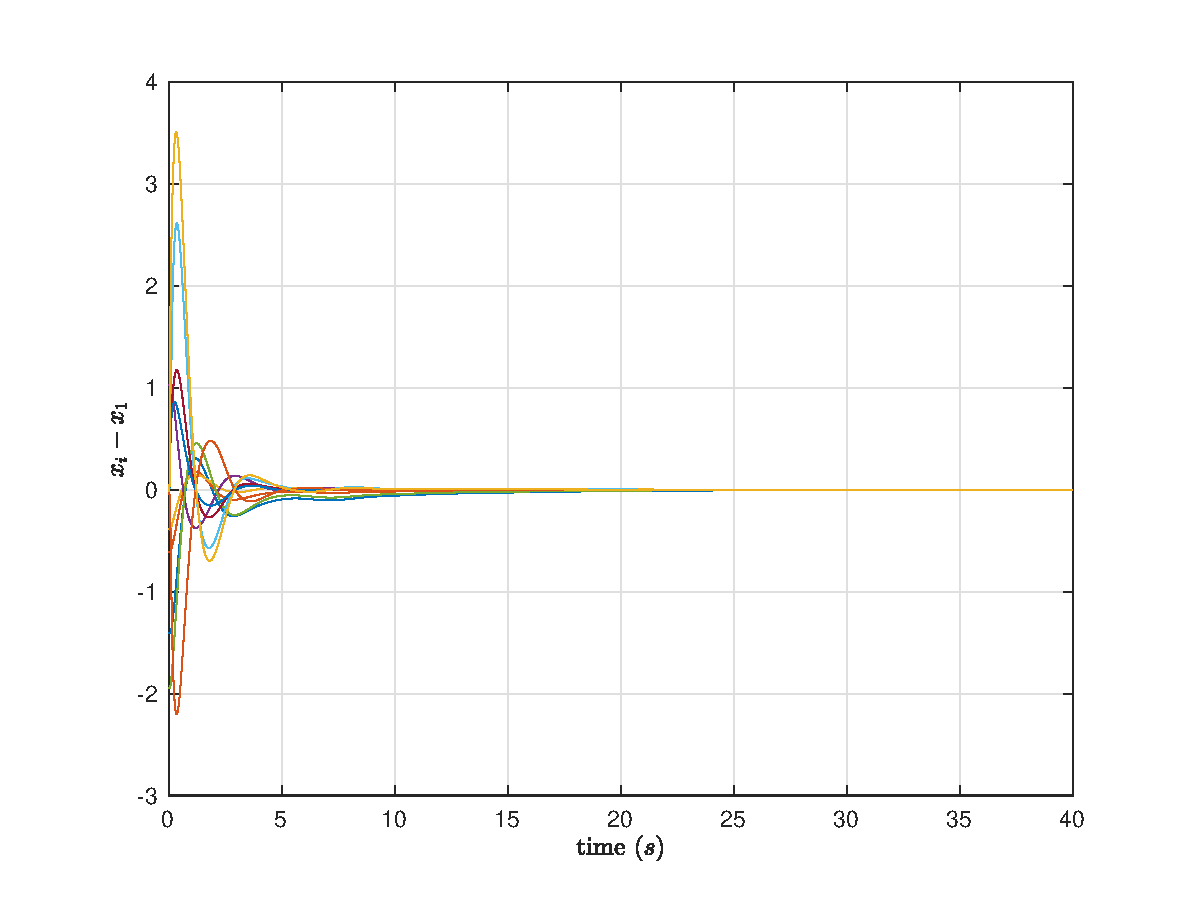
\includegraphics[width=\hsize]{figures/consensus_errors.eps}
  \caption{The consensus errors $x_i-x_1,~~i=1,\cdots, 6$}
  \label{cpic}
\end{figure} 


\begin{figure}[!htb]
  \centering
  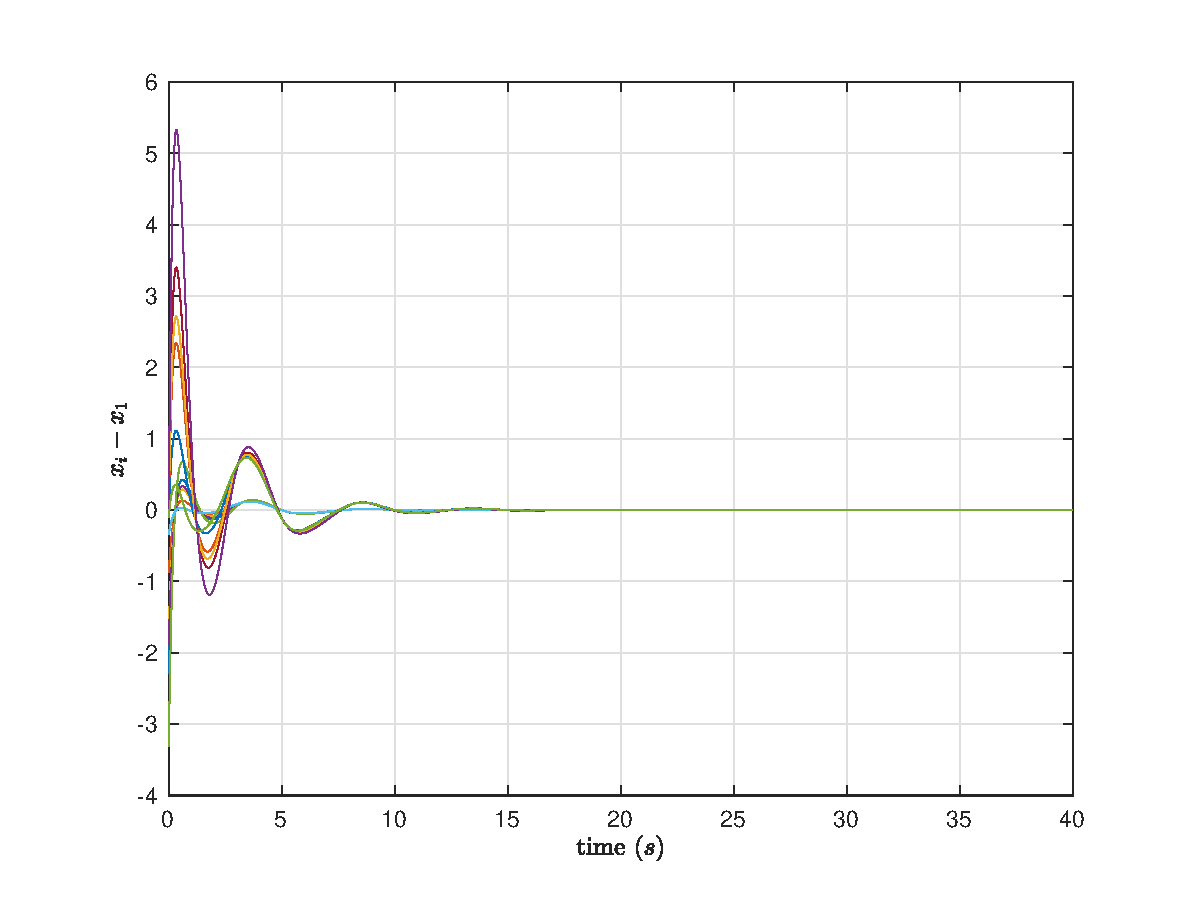
\includegraphics[width=\hsize]{figures/estimation_errors.eps}
  \caption{The observer errors $x_i-\hat x_i,~~i=1,\cdots, 6$}
  \label{epic}
\end{figure}

\section{Conclusion}

The paper has studied the consensus problem of a team of nonlinear agents. Based on linear extended state observer (LESO), we have built a distributed consensus protocol to make the agents achieve consensus. Due to the advantages of node-based adaptive method, the consensus protocols proposed in this paper only need local information of its neighbours, which means they are fully distributed. Finally, the numerical simulation has been provided to demonstrate the validity of the theoretical consequences.


\bibliographystyle{ieeetr}
\bibliography{myreferences}


\end{document}
